\documentclass[pdflatex, sn-nature]{sn-jnl}\usepackage[]{graphicx}\usepackage[]{xcolor}
% maxwidth is the original width if it is less than linewidth
% otherwise use linewidth (to make sure the graphics do not exceed the margin)
\makeatletter
\def\maxwidth{ %
  \ifdim\Gin@nat@width>\linewidth
    \linewidth
  \else
    \Gin@nat@width
  \fi
}
\makeatother

\definecolor{fgcolor}{rgb}{0.345, 0.345, 0.345}
\newcommand{\hlnum}[1]{\textcolor[rgb]{0.686,0.059,0.569}{#1}}%
\newcommand{\hlstr}[1]{\textcolor[rgb]{0.192,0.494,0.8}{#1}}%
\newcommand{\hlcom}[1]{\textcolor[rgb]{0.678,0.584,0.686}{\textit{#1}}}%
\newcommand{\hlopt}[1]{\textcolor[rgb]{0,0,0}{#1}}%
\newcommand{\hlstd}[1]{\textcolor[rgb]{0.345,0.345,0.345}{#1}}%
\newcommand{\hlkwa}[1]{\textcolor[rgb]{0.161,0.373,0.58}{\textbf{#1}}}%
\newcommand{\hlkwb}[1]{\textcolor[rgb]{0.69,0.353,0.396}{#1}}%
\newcommand{\hlkwc}[1]{\textcolor[rgb]{0.333,0.667,0.333}{#1}}%
\newcommand{\hlkwd}[1]{\textcolor[rgb]{0.737,0.353,0.396}{\textbf{#1}}}%
\let\hlipl\hlkwb

\usepackage{framed}
\makeatletter
\newenvironment{kframe}{%
 \def\at@end@of@kframe{}%
 \ifinner\ifhmode%
  \def\at@end@of@kframe{\end{minipage}}%
  \begin{minipage}{\columnwidth}%
 \fi\fi%
 \def\FrameCommand##1{\hskip\@totalleftmargin \hskip-\fboxsep
 \colorbox{shadecolor}{##1}\hskip-\fboxsep
     % There is no \\@totalrightmargin, so:
     \hskip-\linewidth \hskip-\@totalleftmargin \hskip\columnwidth}%
 \MakeFramed {\advance\hsize-\width
   \@totalleftmargin\z@ \linewidth\hsize
   \@setminipage}}%
 {\par\unskip\endMakeFramed%
 \at@end@of@kframe}
\makeatother

\definecolor{shadecolor}{rgb}{.97, .97, .97}
\definecolor{messagecolor}{rgb}{0, 0, 0}
\definecolor{warningcolor}{rgb}{1, 0, 1}
\definecolor{errorcolor}{rgb}{1, 0, 0}
\newenvironment{knitrout}{}{} % an empty environment to be redefined in TeX

\usepackage{alltt}

\usepackage{xr}
\usepackage{fullpage}
\usepackage{amsmath}
\usepackage{url}
\usepackage{booktabs}
\usepackage{placeins}

\usepackage[font=small]{caption}

\externaldocument[main-]{../main/future_hail}

%\urlstyle{same}
\newcommand{\degr}{$^{\circ{}}$C}

\renewcommand{\figurename}{Extended Data Figure}
\renewcommand\refname{Extended Data}
\IfFileExists{upquote.sty}{\usepackage{upquote}}{}
\begin{document}

\title{Shifting hail hazard under global warming and effects on crop hail exposure: extended data}

\author*[1,2,3,4]{\fnm{Timothy H.} \sur{Raupach}}\email{timothy.h.raupach@gmail.com}
\author[5,6]{\fnm{Raphael} \sur{Portmann}}
\author[7]{\fnm{Christian} \sur{Siderius}}
\author[2,3,4]{\fnm{Steven C.} \sur{Sherwood}}

\affil[1]{\orgdiv{Institute for Climate Risk and Response}, \orgname{UNSW Sydney}, \orgaddress{\street{Mathews Building Level 4}, \city{The University of New South Wales, Sydney}, \postcode{2051}, \state{NSW}, \country{Australia}}}
\affil[2]{\orgdiv{Climate Change Research Centre}, \orgname{UNSW Sydney}, \orgaddress{\country{Australia}}}
\affil[3]{\orgdiv{ARC Centre of Excellence for Climate Extremes}, \orgname{UNSW Sydney}, \orgaddress{\country{Australia}}}
\affil[4]{\orgdiv{ARC Centre of Excellence for 21st Century Weather}, \orgname{UNSW Sydney}, \orgaddress{\country{Australia}}}
\affil[5]{\orgdiv{Agroscope}, \orgname{Swiss Federal Office for Agriculture}, \orgaddress{\city{Zurich}, \country{Switzerland (prev. address)}}}
\affil[6]{\orgname{Planval}, \orgaddress{\city{Bern}, \country{Switzerland}}}
\affil[7]{\orgname{Uncharted Waters}, \orgaddress{\city{Sydney}, \country{Australia}}}

\maketitle

\begin{figure*}[p]
    \centering
    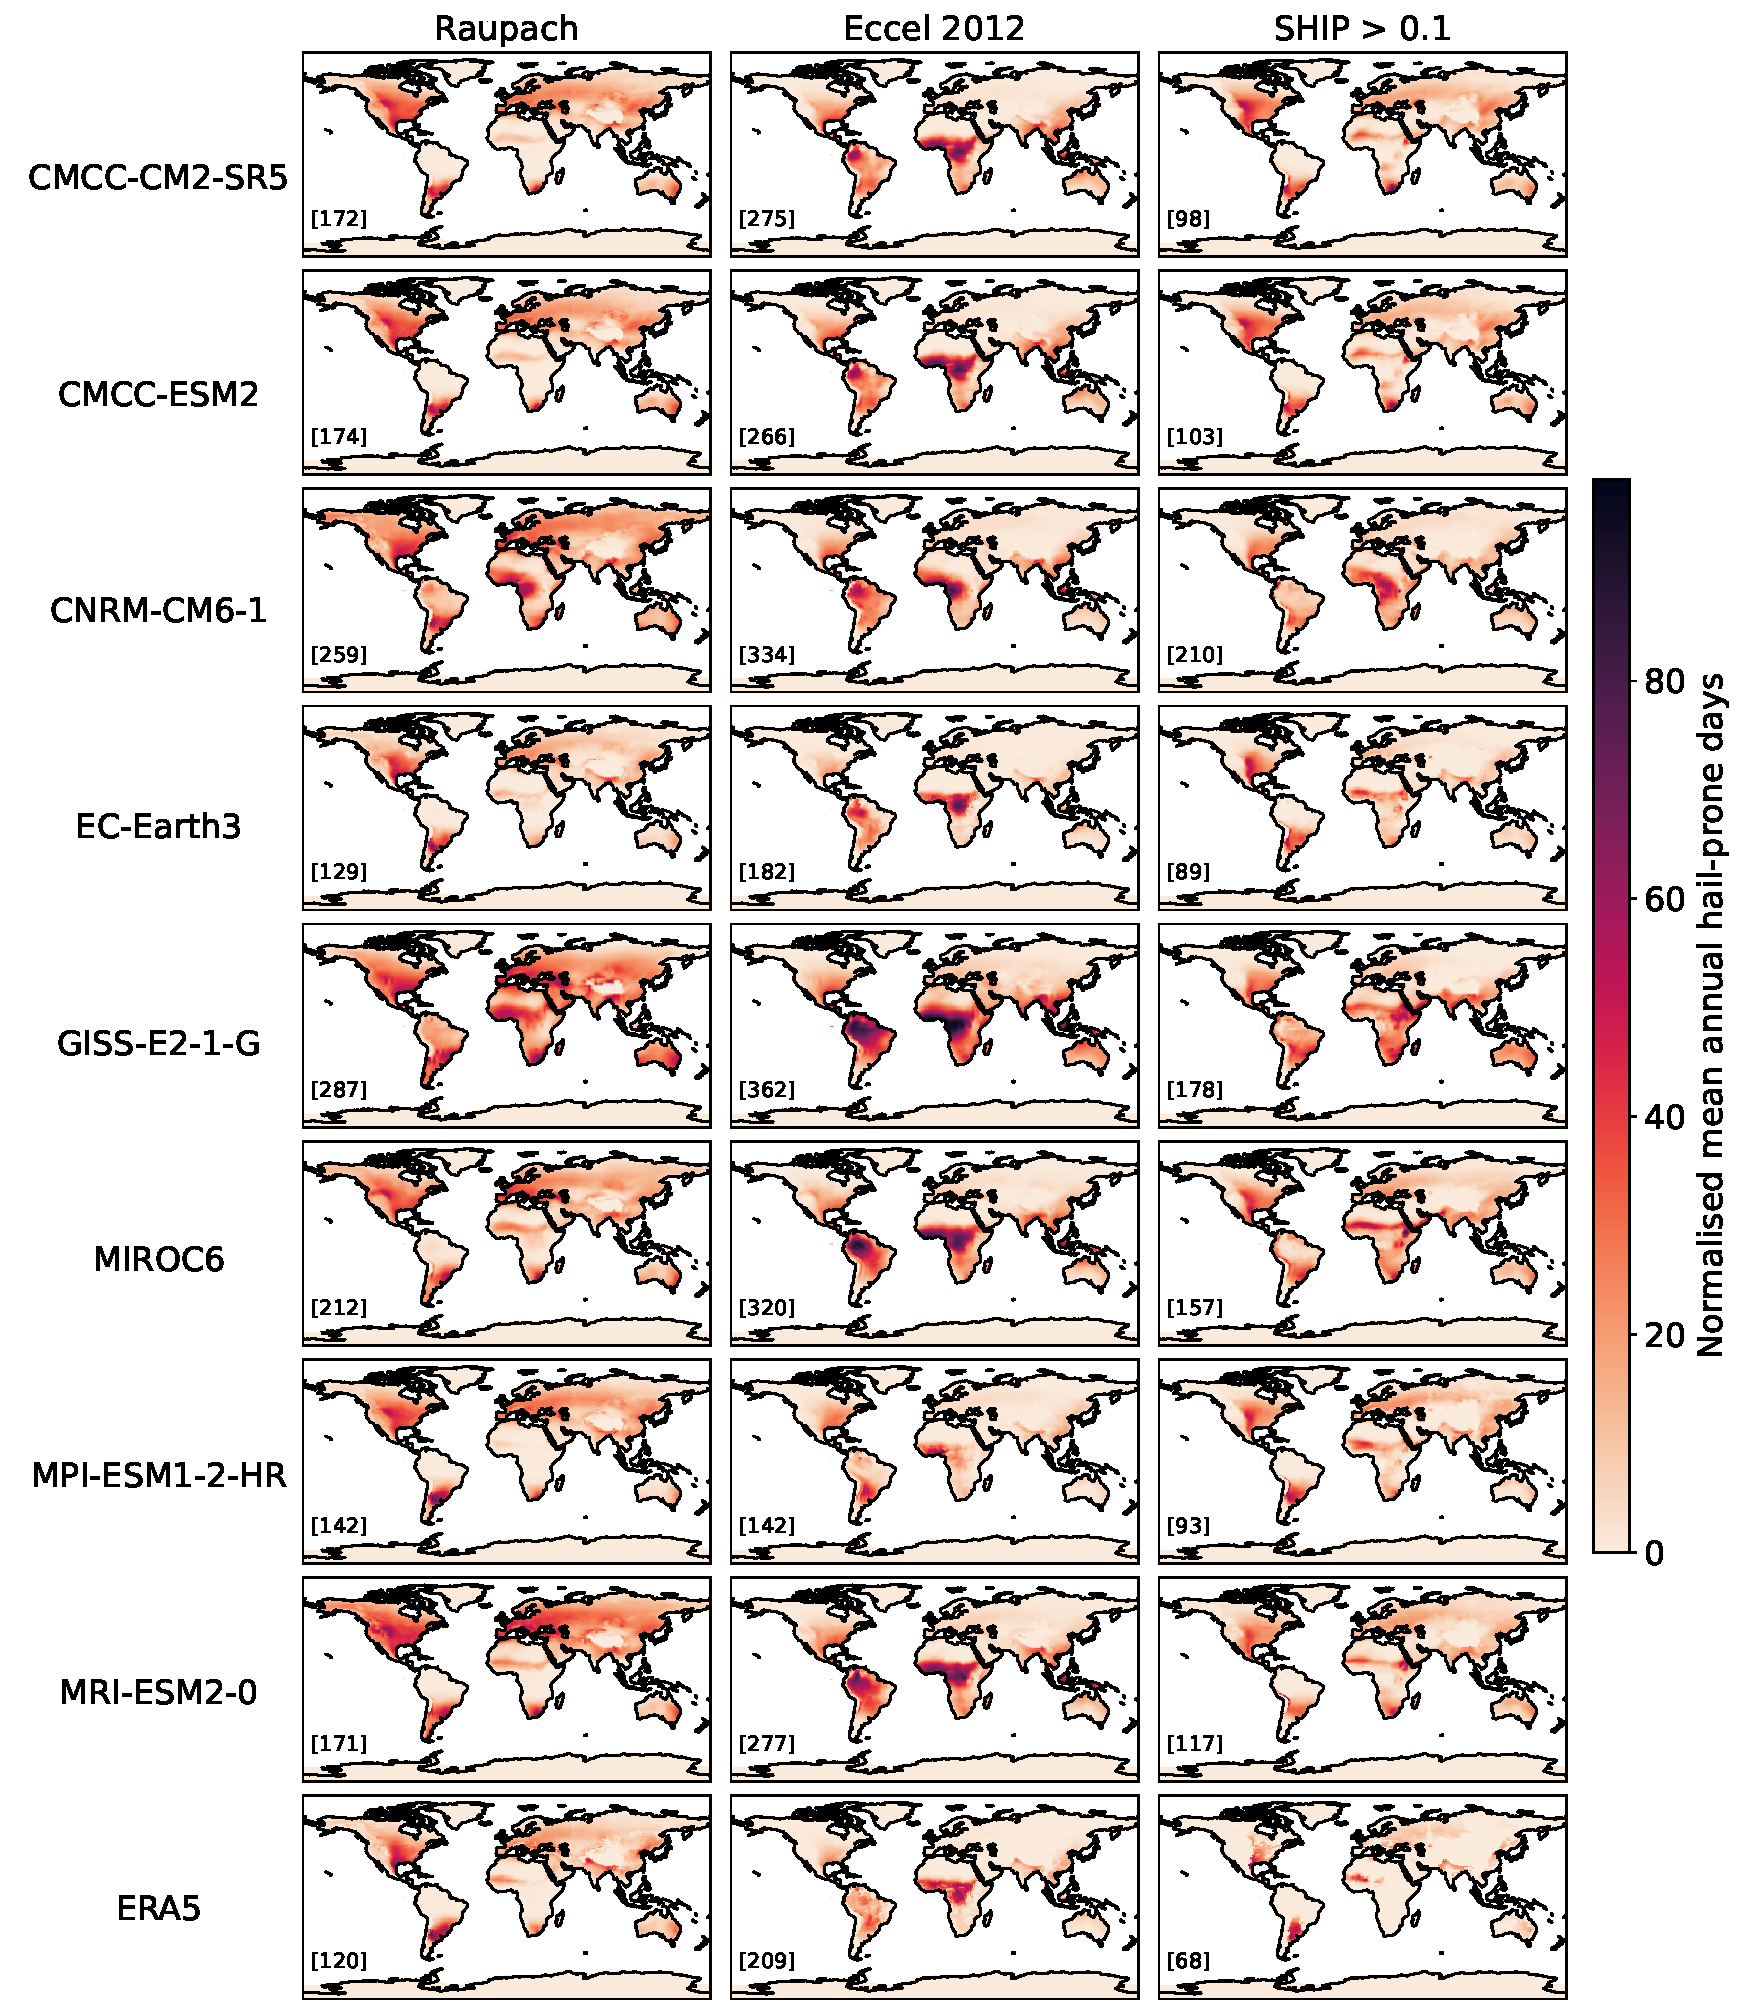
\includegraphics[width=\textwidth]{../../results/extended_data/historical_by_model}
    \caption{\textbf{Mean annual hail-prone days in historical (1980-1999)
    runs.} There is one row per model (each CMIP6 model and ERA5 reanalysis),
    and one column per proxy. Inset numbers in square brackets show the normalisation factor by which each map was scaled, the maximum annual hail-prone days over the historical period.}
    \label{fig:historical_annual_means}
\end{figure*}

\begin{figure*}[h]
    \centering
    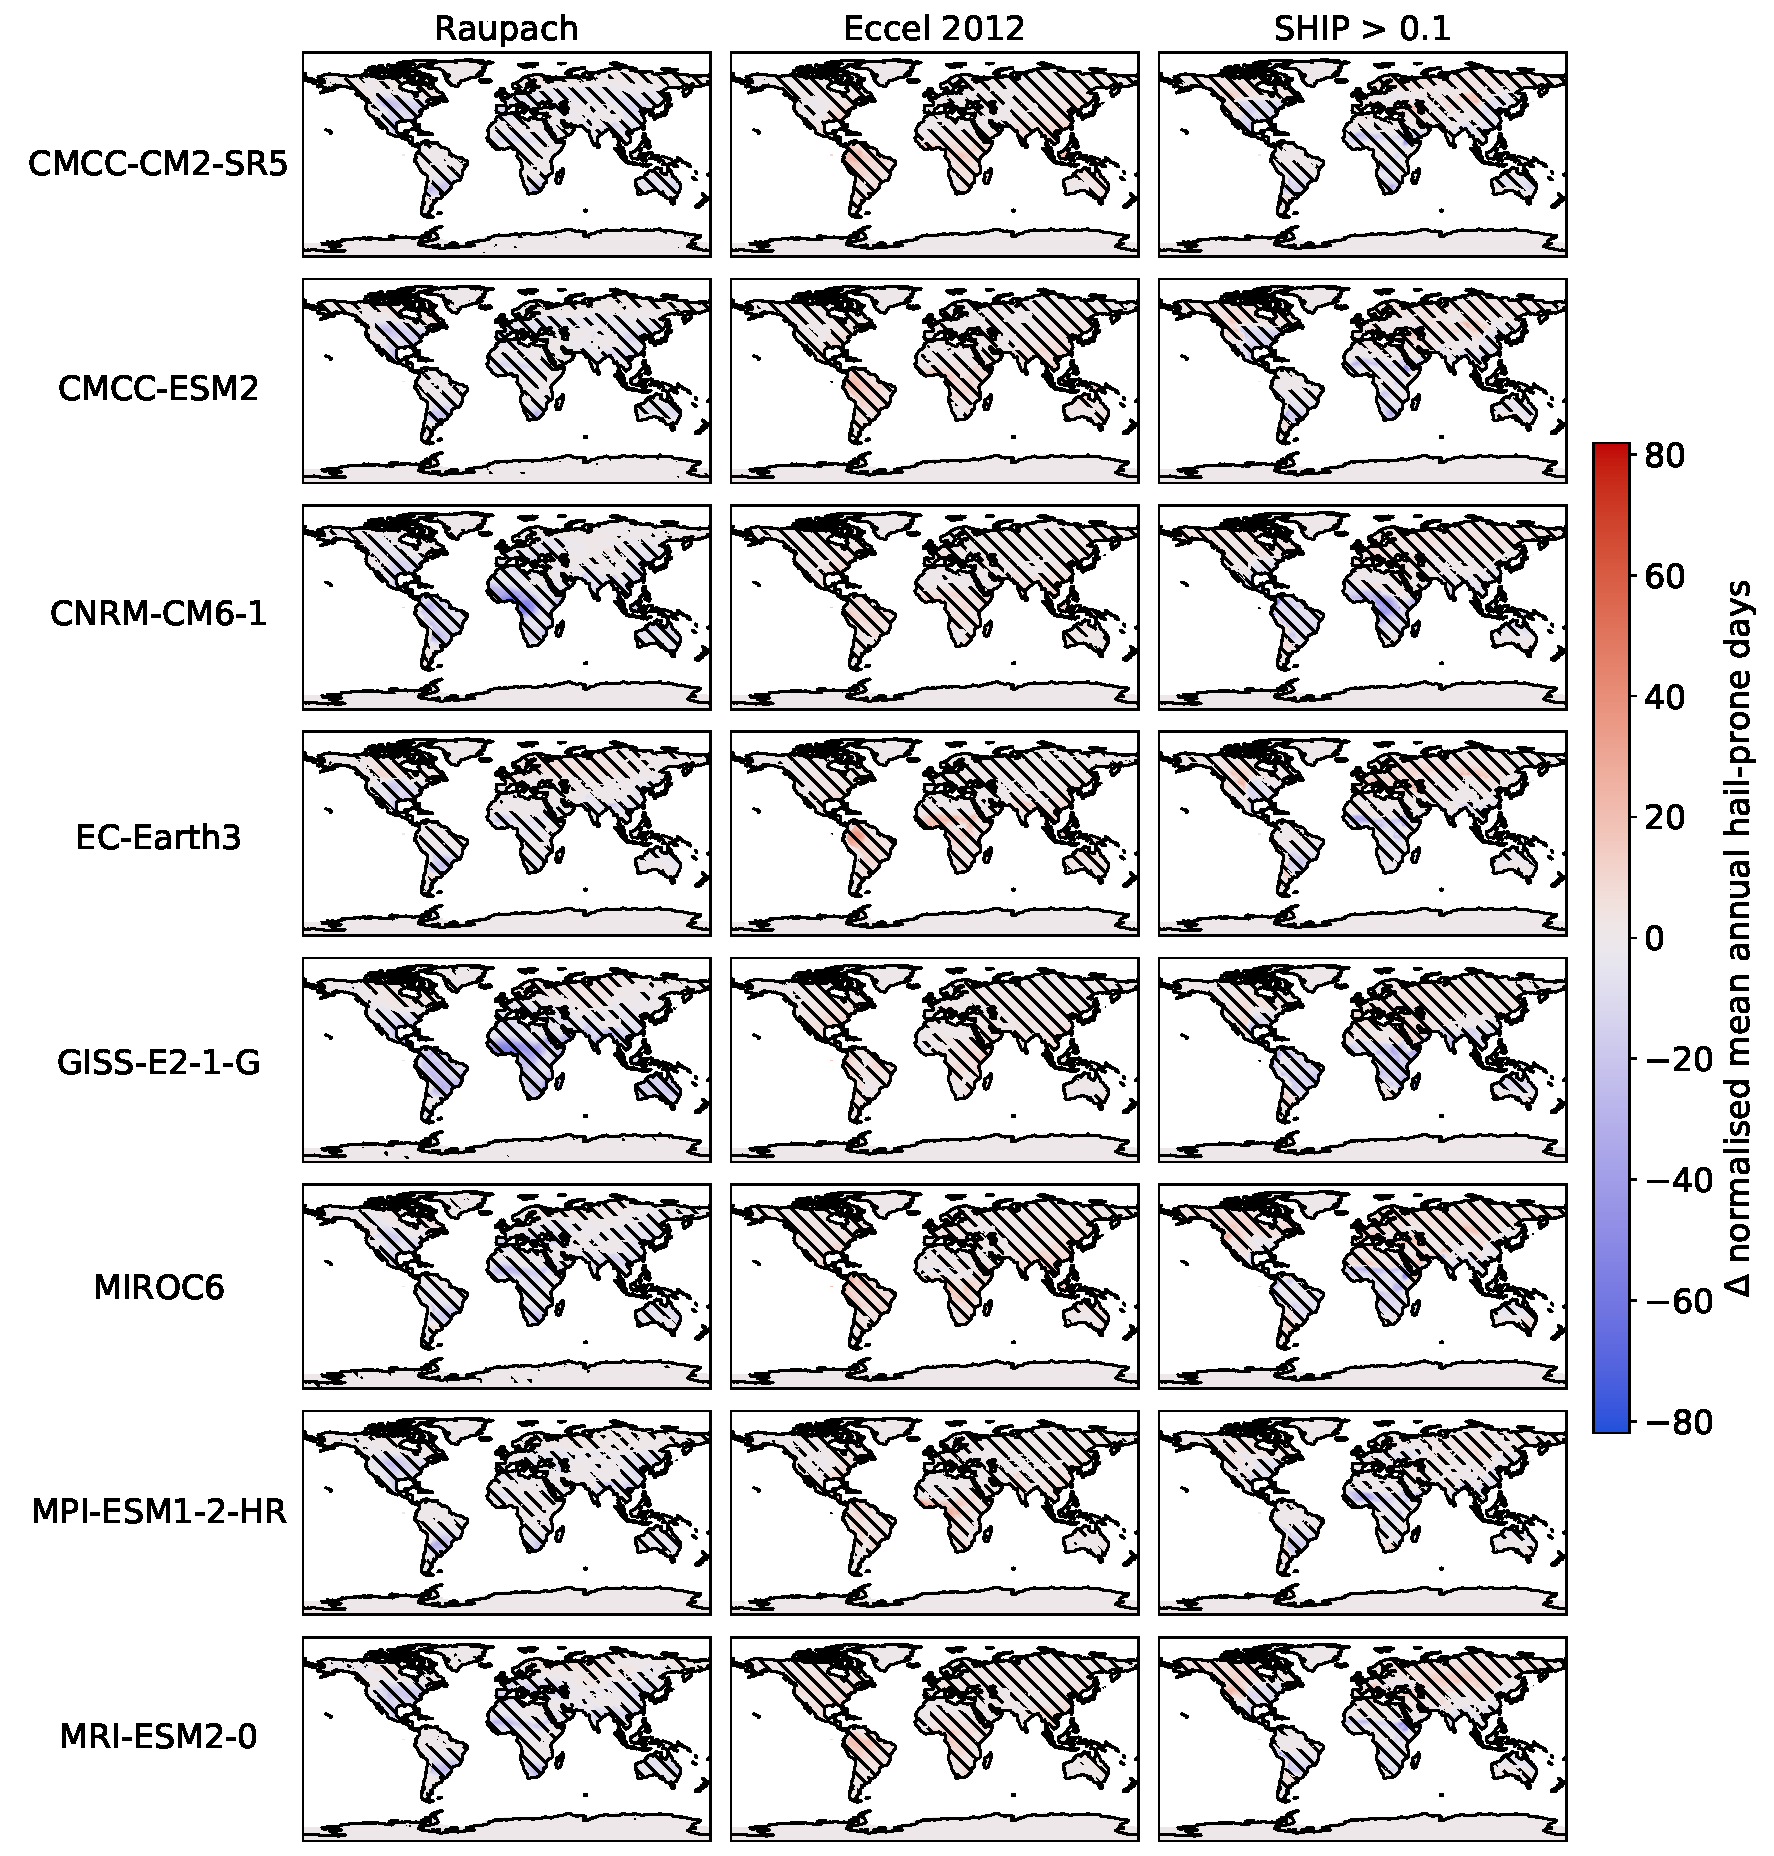
\includegraphics[width=\textwidth]{../../results/extended_data/hail_diffs_3C}
    \caption{\textbf{Differences in mean annual hail-prone days by model and
    proxy for 3 \degr{} global warming.} Stippling shows regions for which the
    difference between epochs was statistically significant ($p <$ 0.05 using
    Welch's t-test).}
    \label{fig:hail_diffs_3C}
\end{figure*}

\begin{figure*}[h]
    \centering
    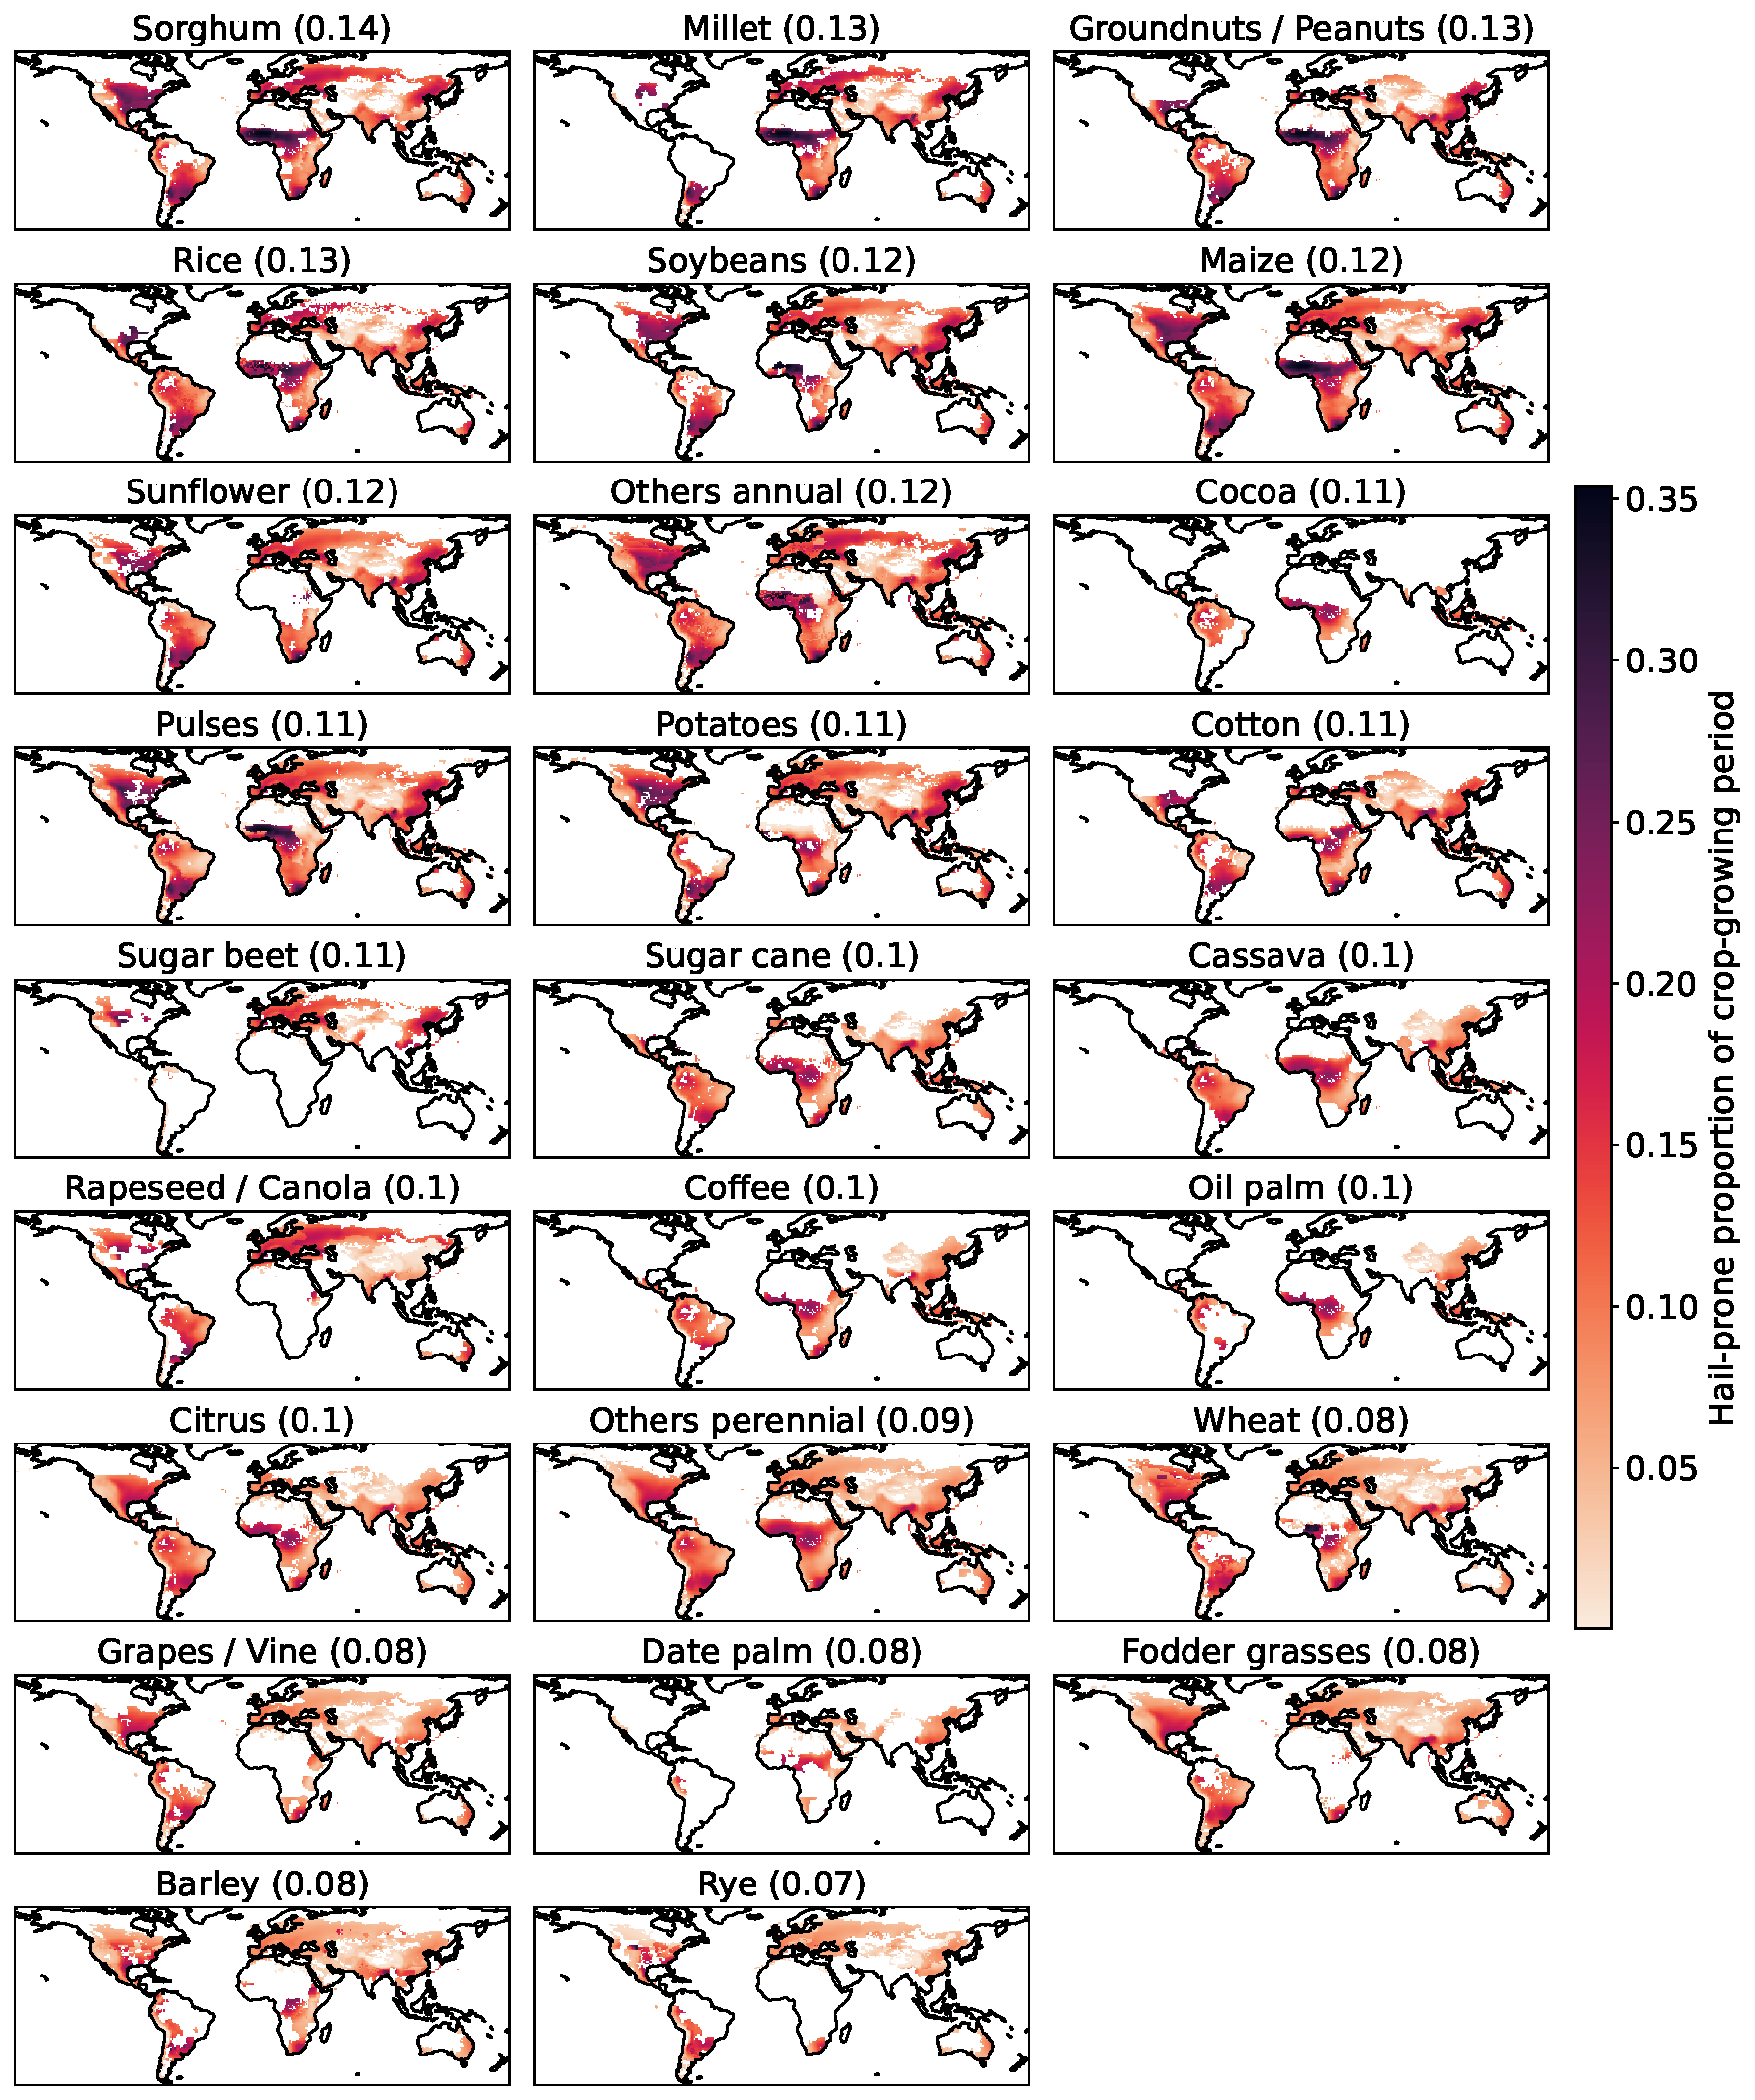
\includegraphics[width=\textwidth]{../../results/extended_data/historical_crop_proportion_hail_prone}
    \caption{\textbf{Multimodel, multi-proxy mean hail-prone proportions of
    cropping seasons for the historical period.} Brackets in titles show overall
    mean hail-prone proportion of cropping seasons by crop. Plots are subset to
    remove areas with no crop data.}
    \label{fig:historic_crop_proportions}
\end{figure*}

\begin{figure*}[h]
    \centering
    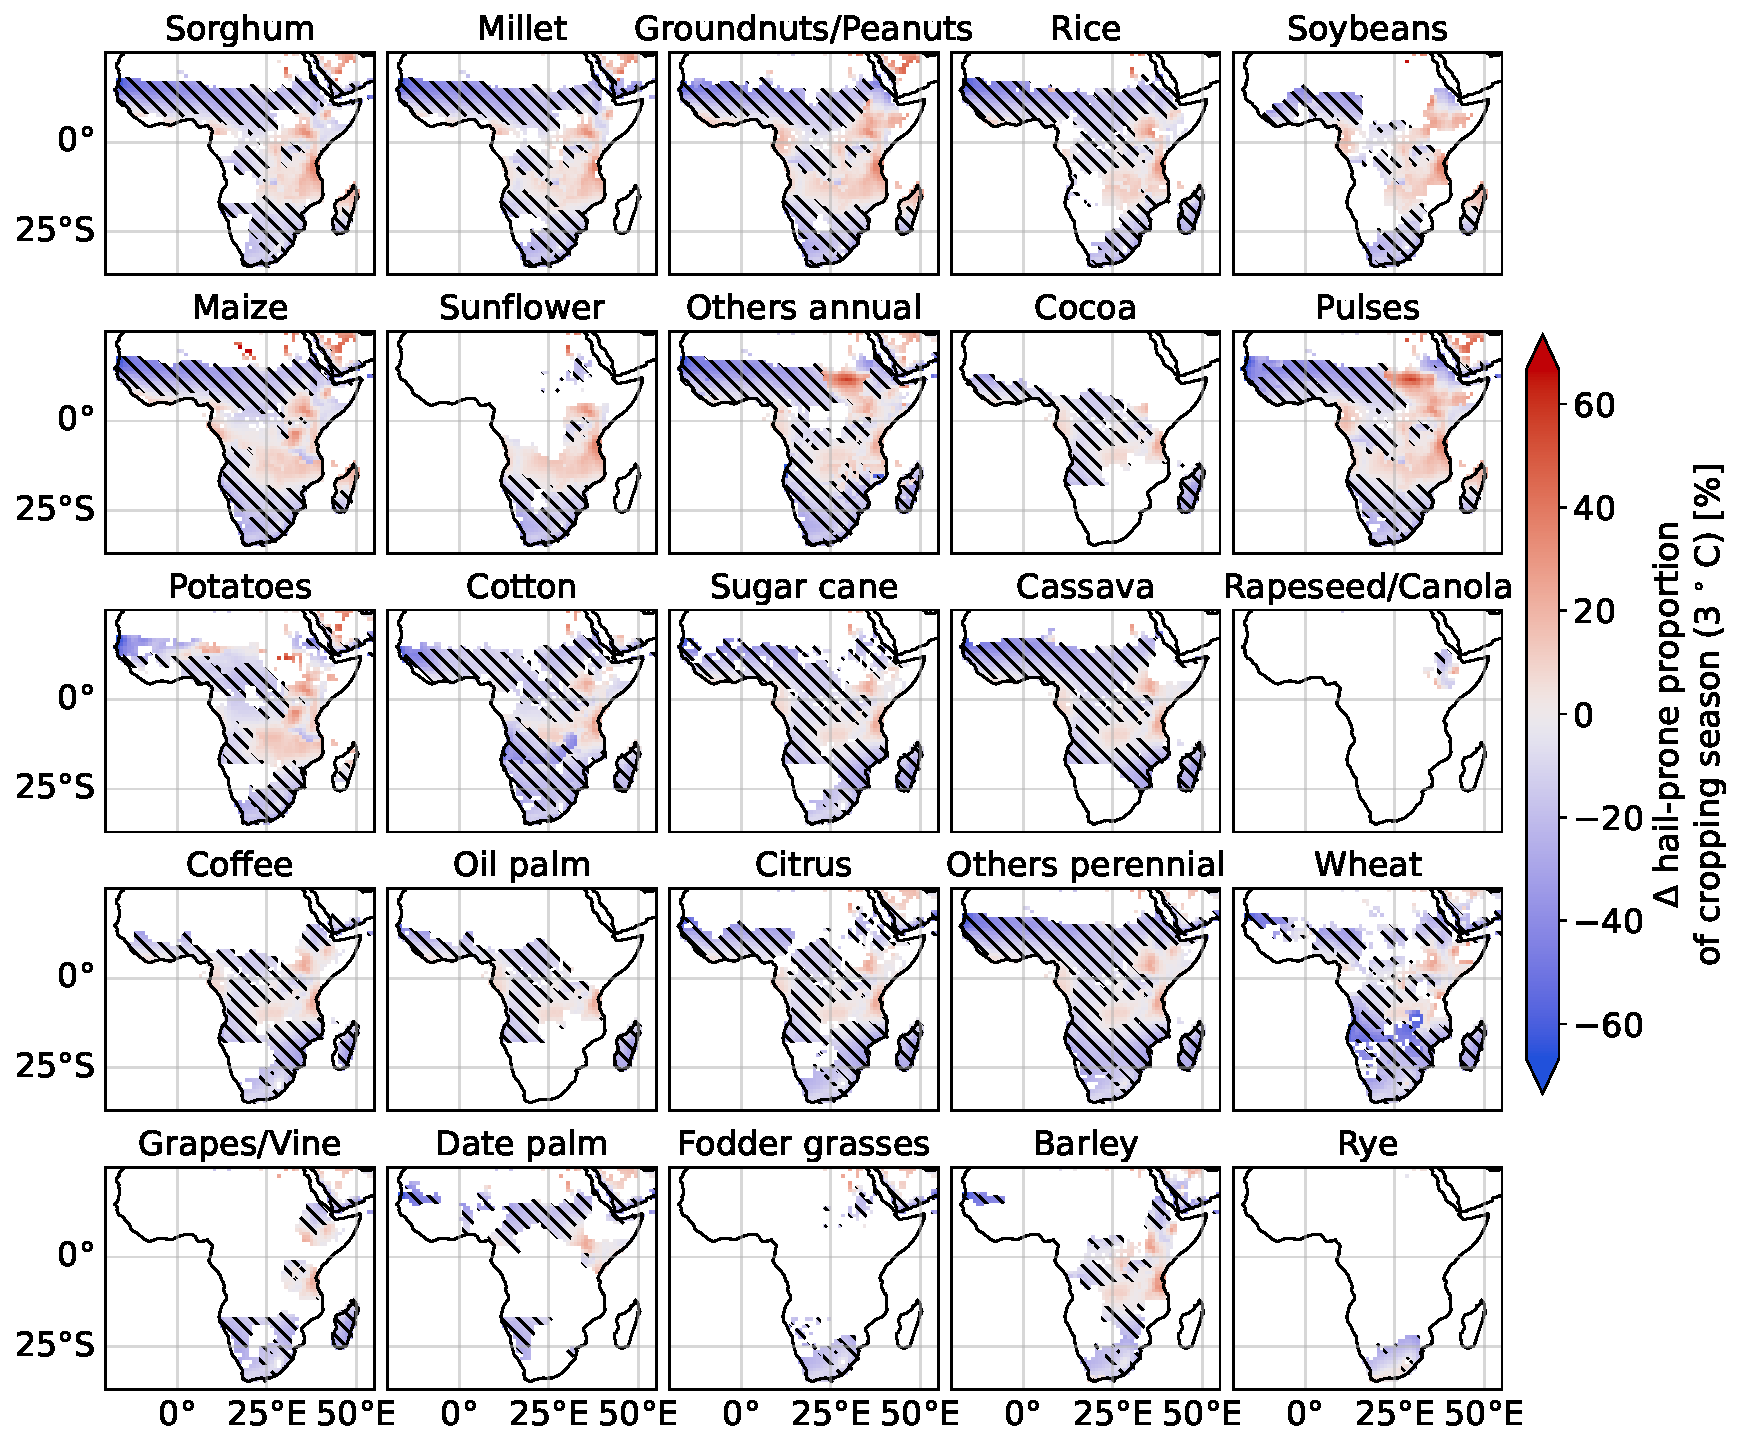
\includegraphics[width=\textwidth]{../../results/extended_data/crop_changes_africa}
    \caption{\textbf{Regional, relative changes in hail-prone proportion of
    cropping season}. Multimodel, multi-proxy mean change in hail-prone
    proportions of cropping seasons for 3 \degr{} warming, for Africa, with
    changes shown as percentages of the historical hail-prone proportion of
    cropping season. Crops for which there were no significant changes recorded
    are not shown. Stippling shows regions in which at least 50\% of the
    model/proxy combinations agreed with the sign of the mean difference and
    also showed significant differences in the mean ($p < 0.05$ on a t-test on
    two related samples). The colour bar is truncated to the range of stippled
    values and is non-linear with zero at the centre.}
    \label{fig:crop_changes_africa}
\end{figure*}

\begin{figure*}[h]
    \centering
    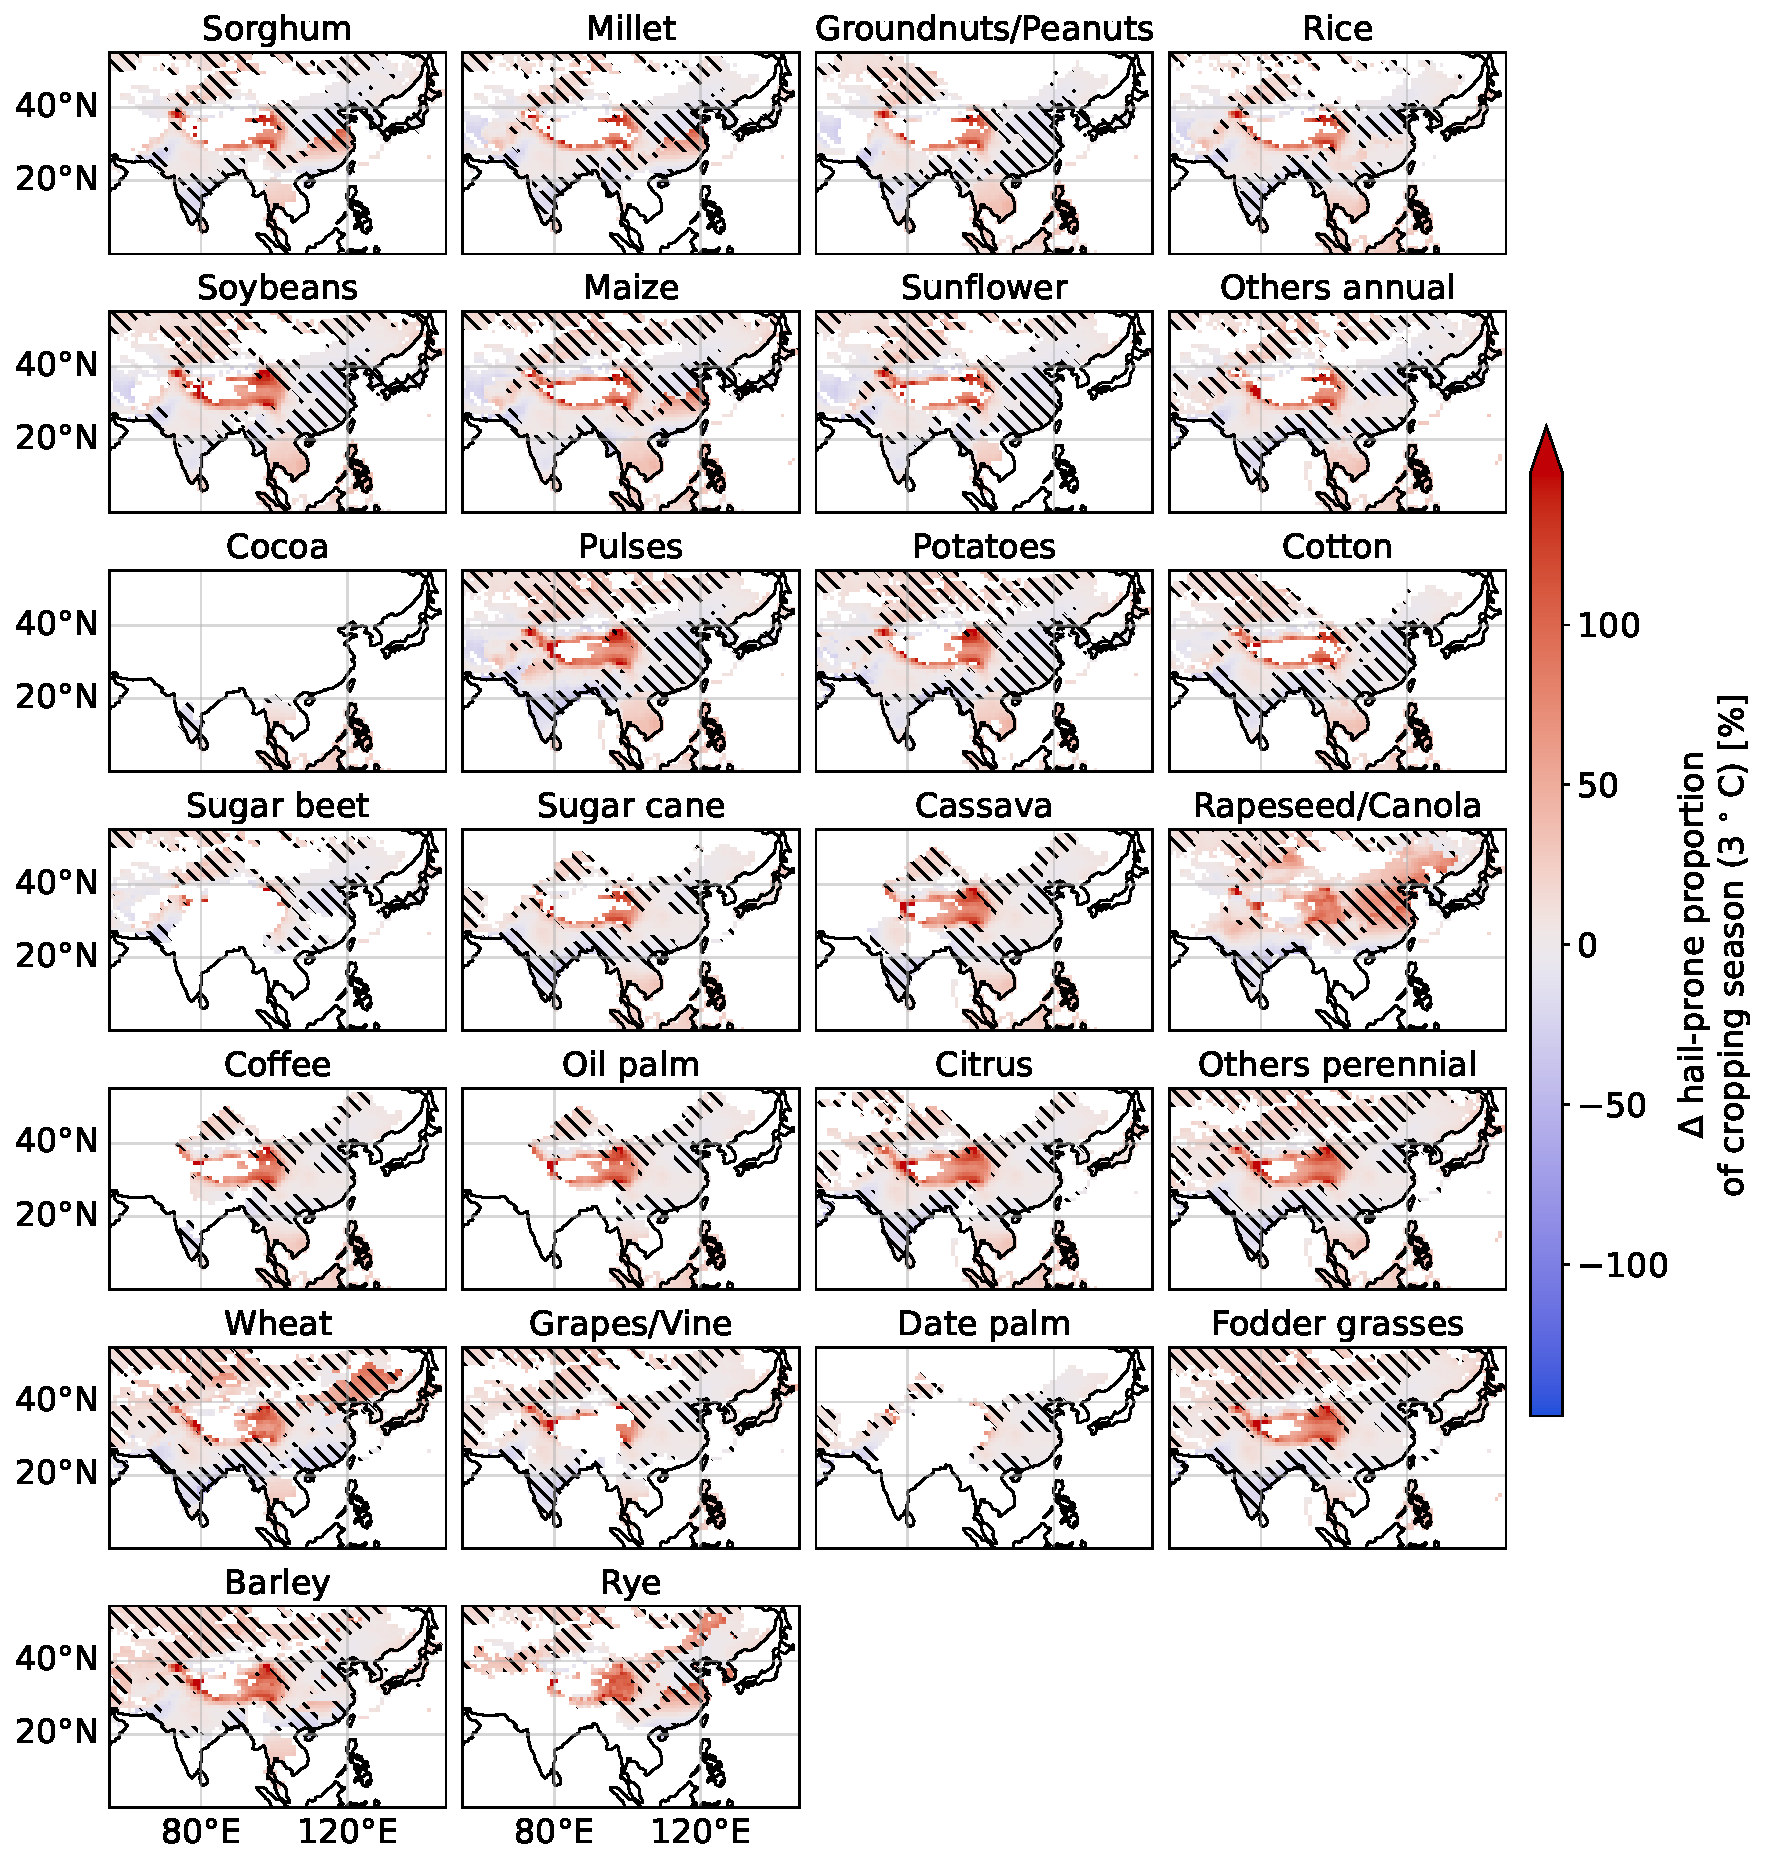
\includegraphics[width=\textwidth]{../../results/extended_data/crop_changes_asia}
    \caption{As for Extended Data Figure \ref{fig:crop_changes_africa} but for
    Asia.}
    \label{fig:crop_changes_asia}
\end{figure*}

\begin{figure*}[h]
    \centering
    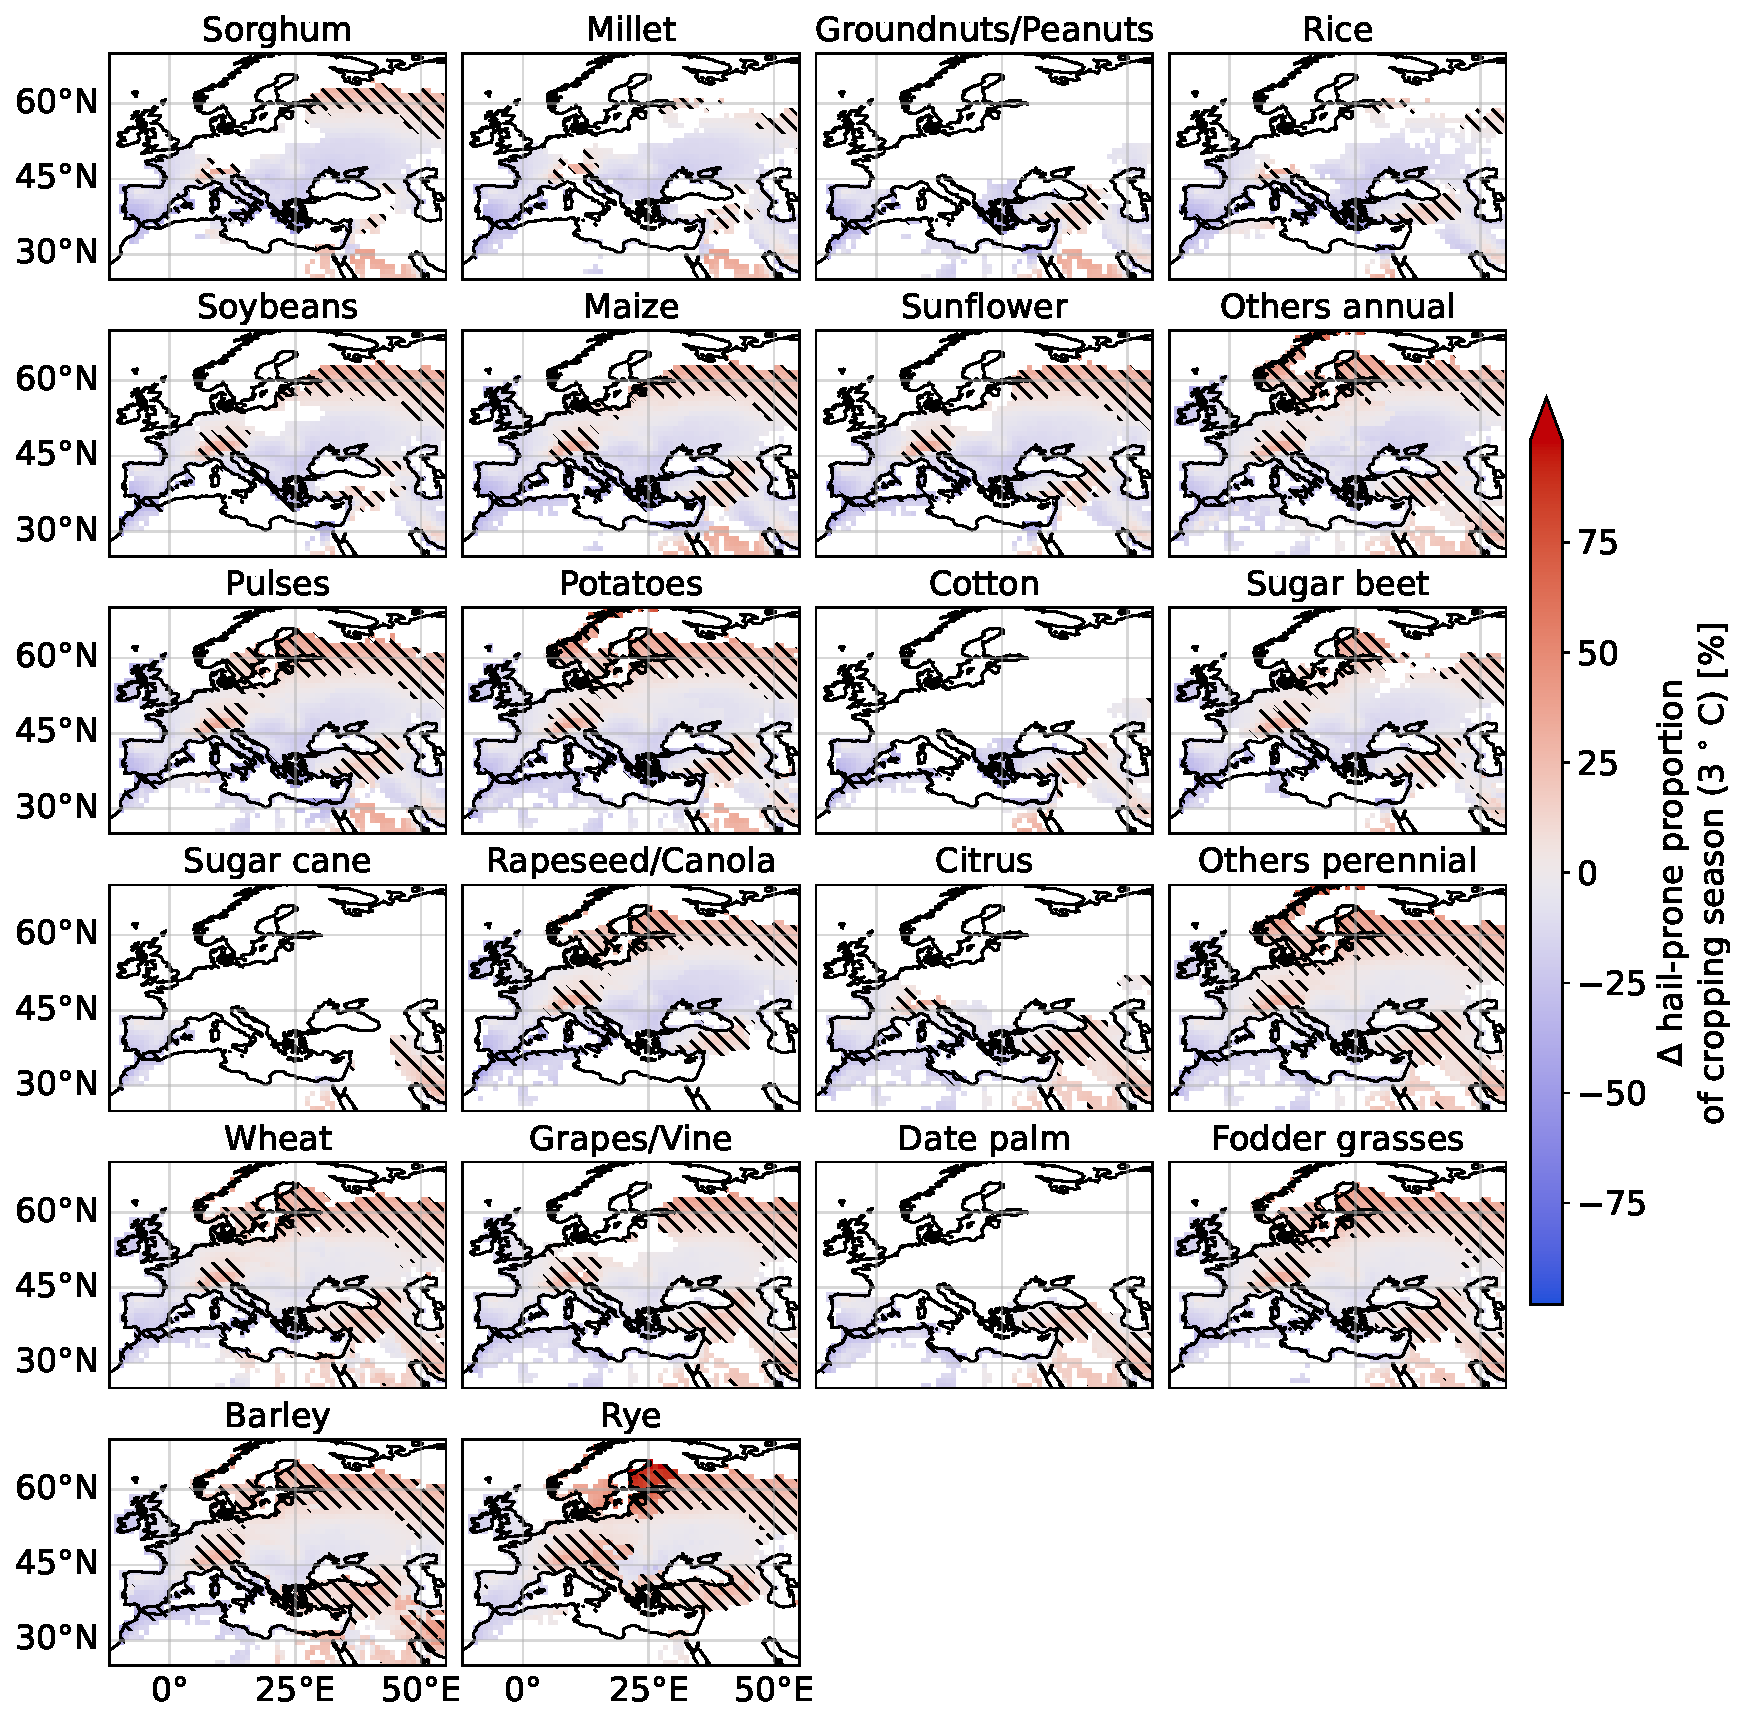
\includegraphics[width=\textwidth]{../../results/extended_data/crop_changes_europe}
    \caption{As for Extended Data Figure \ref{fig:crop_changes_africa} but for
    Europe.}
    \label{fig:crop_changes_europe}
\end{figure*}

\begin{figure*}[h]
    \centering
    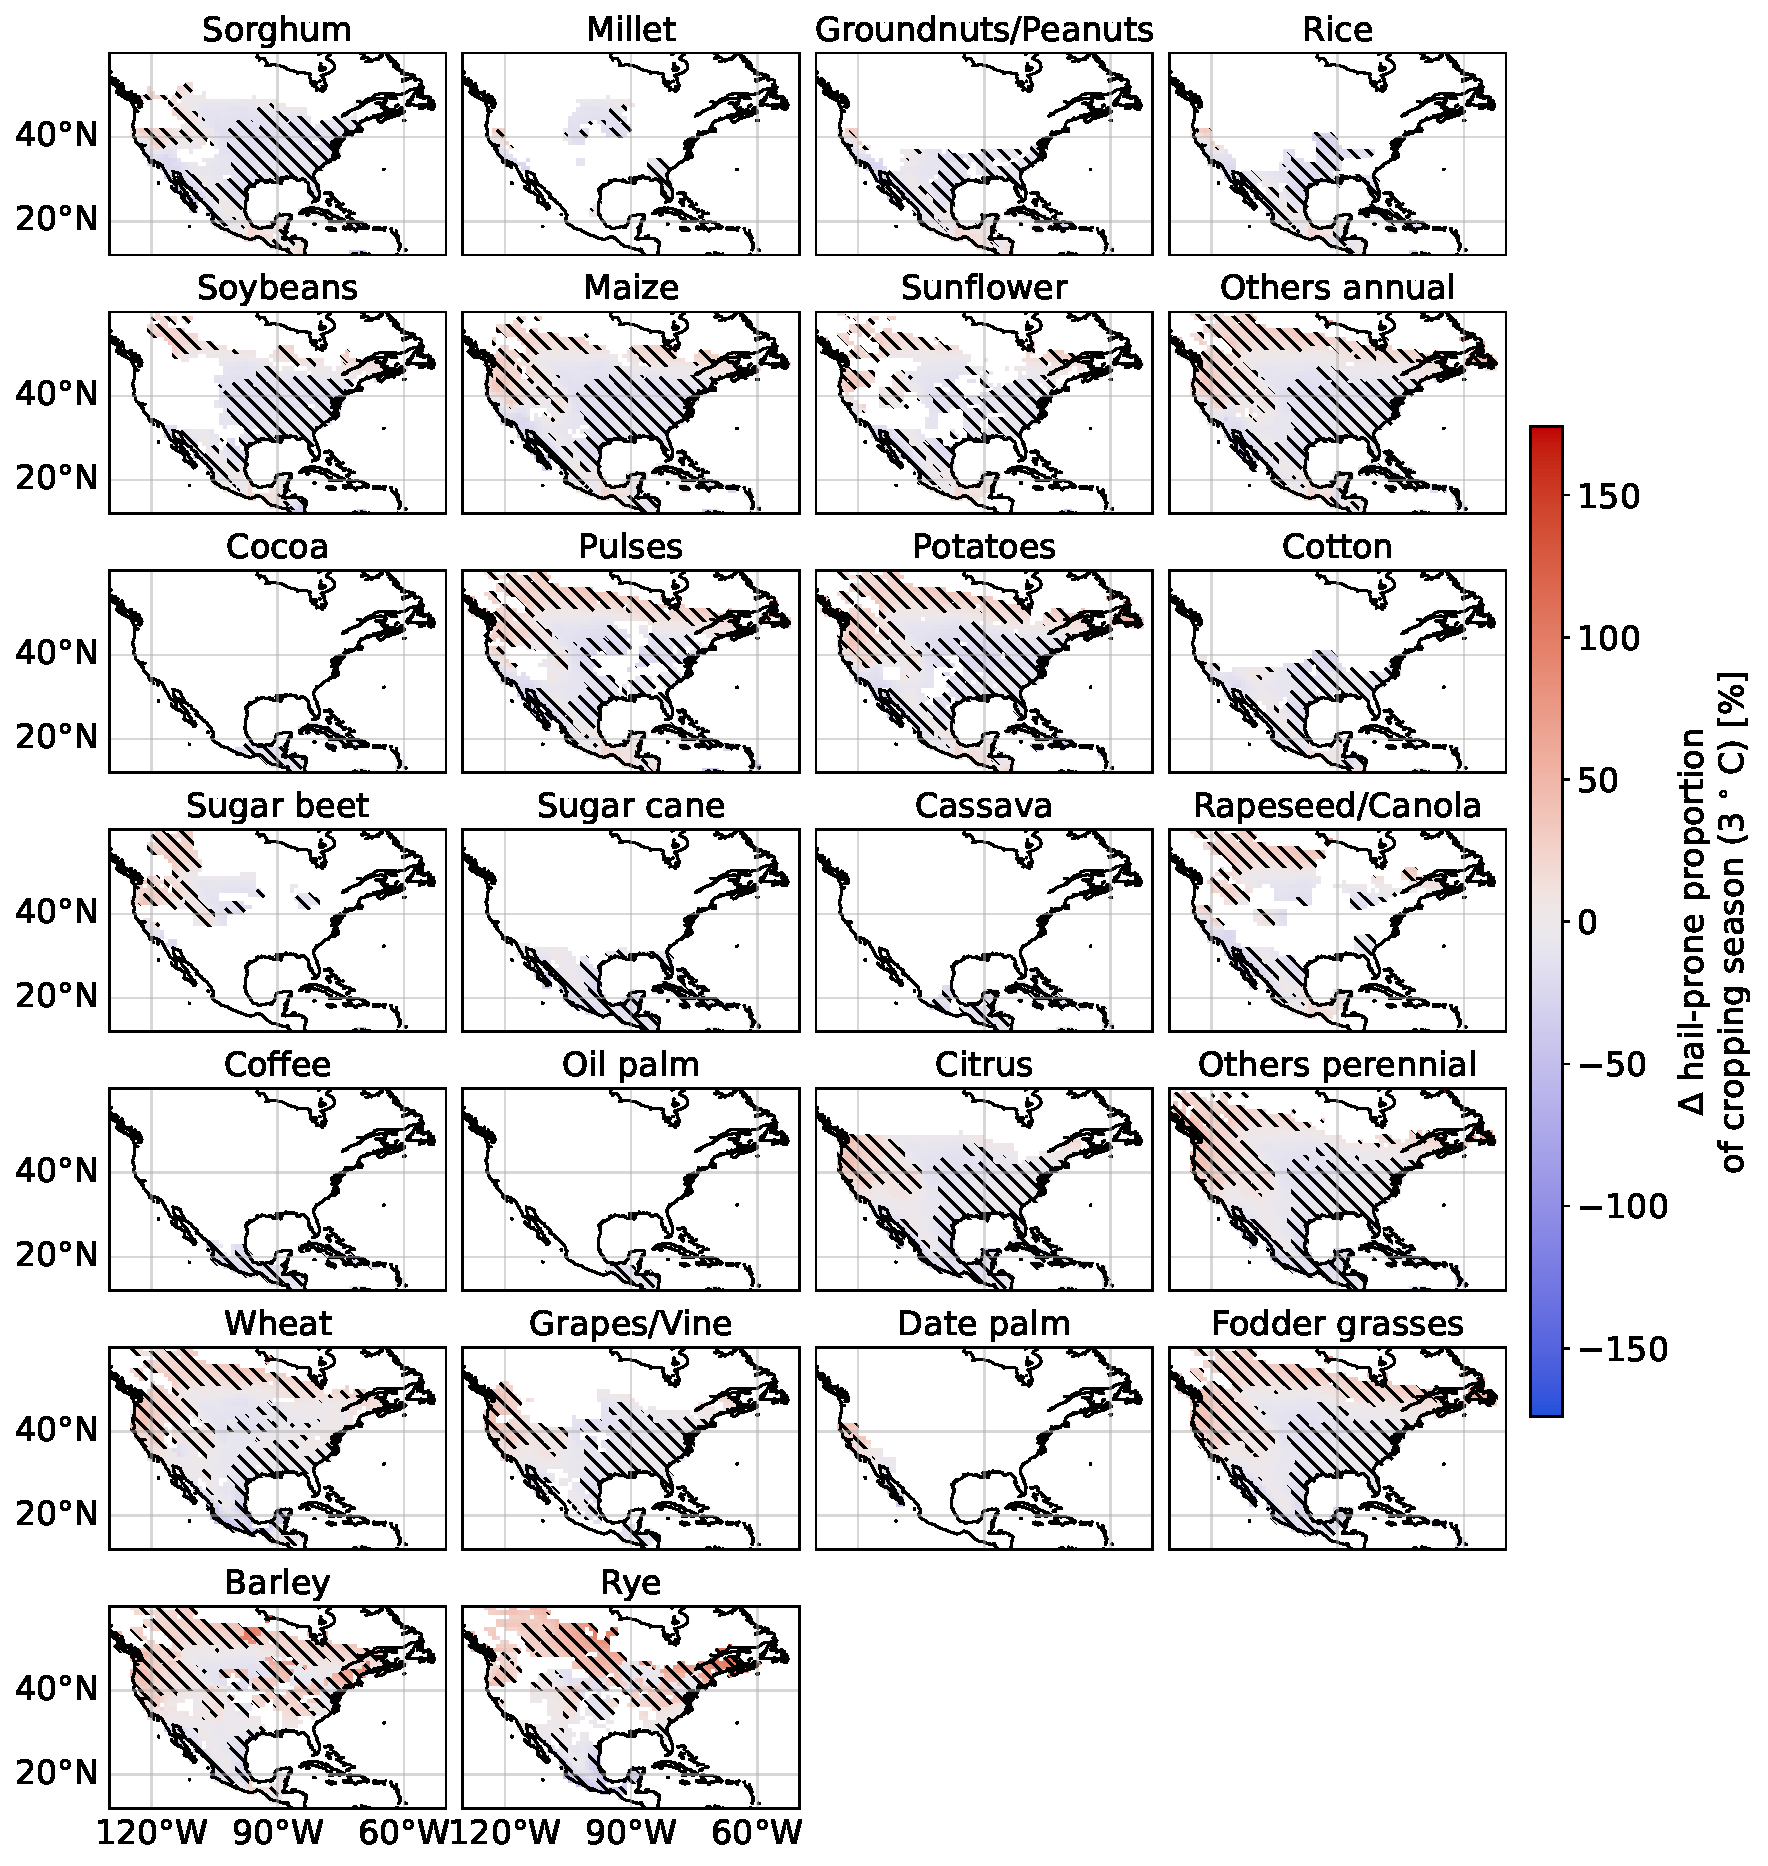
\includegraphics[width=\textwidth]{../../results/extended_data/crop_changes_north_america}
    \caption{As for Extended Data Figure \ref{fig:crop_changes_africa} but for
    North America.}
    \label{fig:crop_changes_north_america}
\end{figure*}

\begin{figure*}[h]
    \centering
    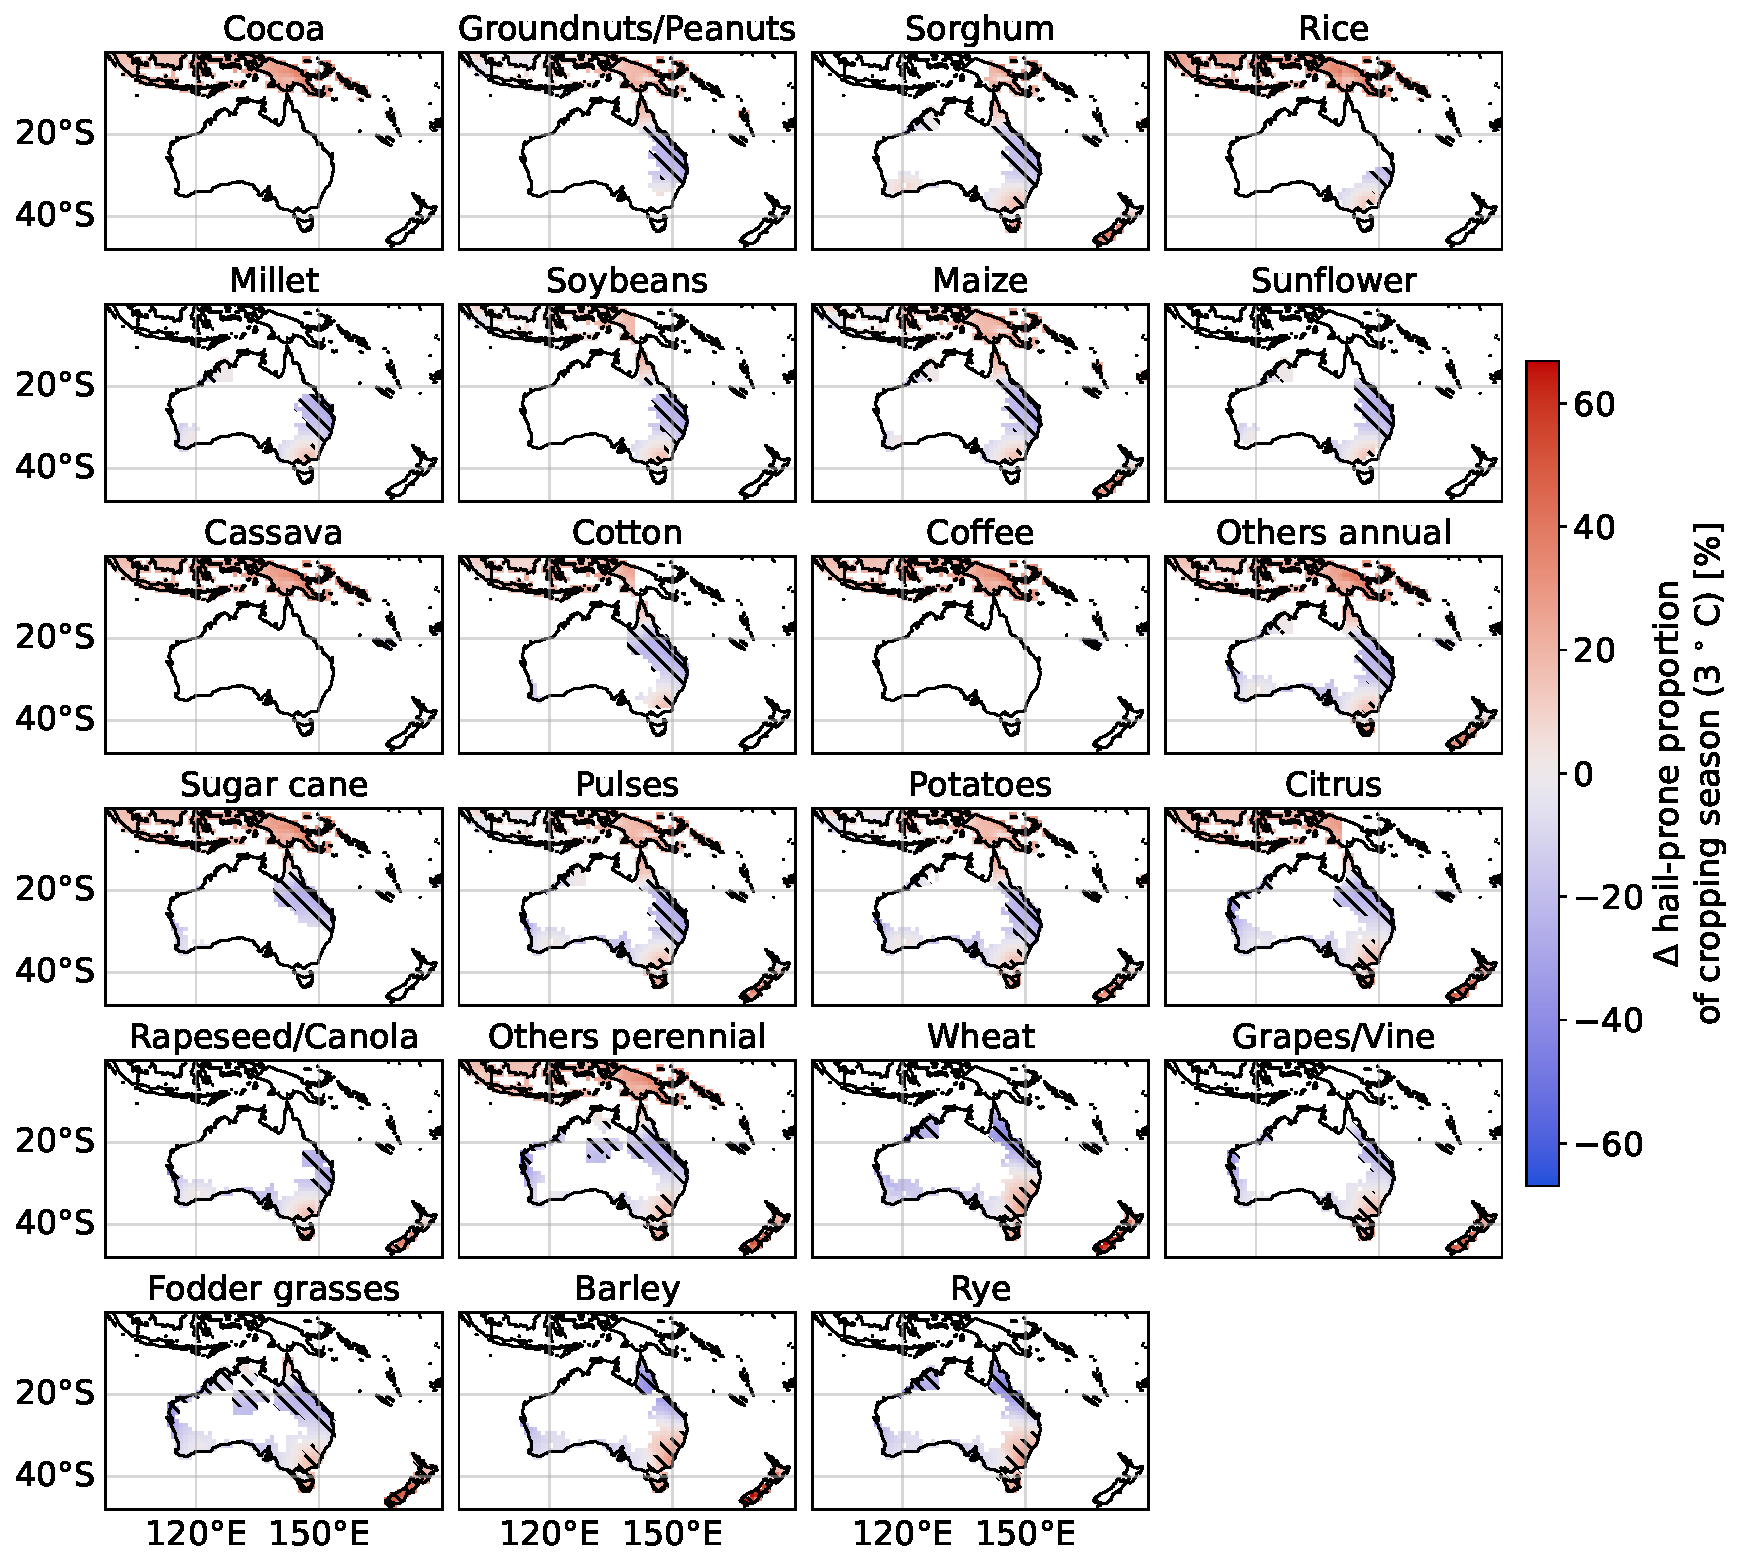
\includegraphics[width=\textwidth]{../../results/extended_data/crop_changes_oceania}
    \caption{As for Extended Data Figure \ref{fig:crop_changes_africa} but for
    Oceania.}
    \label{fig:crop_changes_oceania}
\end{figure*}

\begin{figure*}[h]
    \centering
    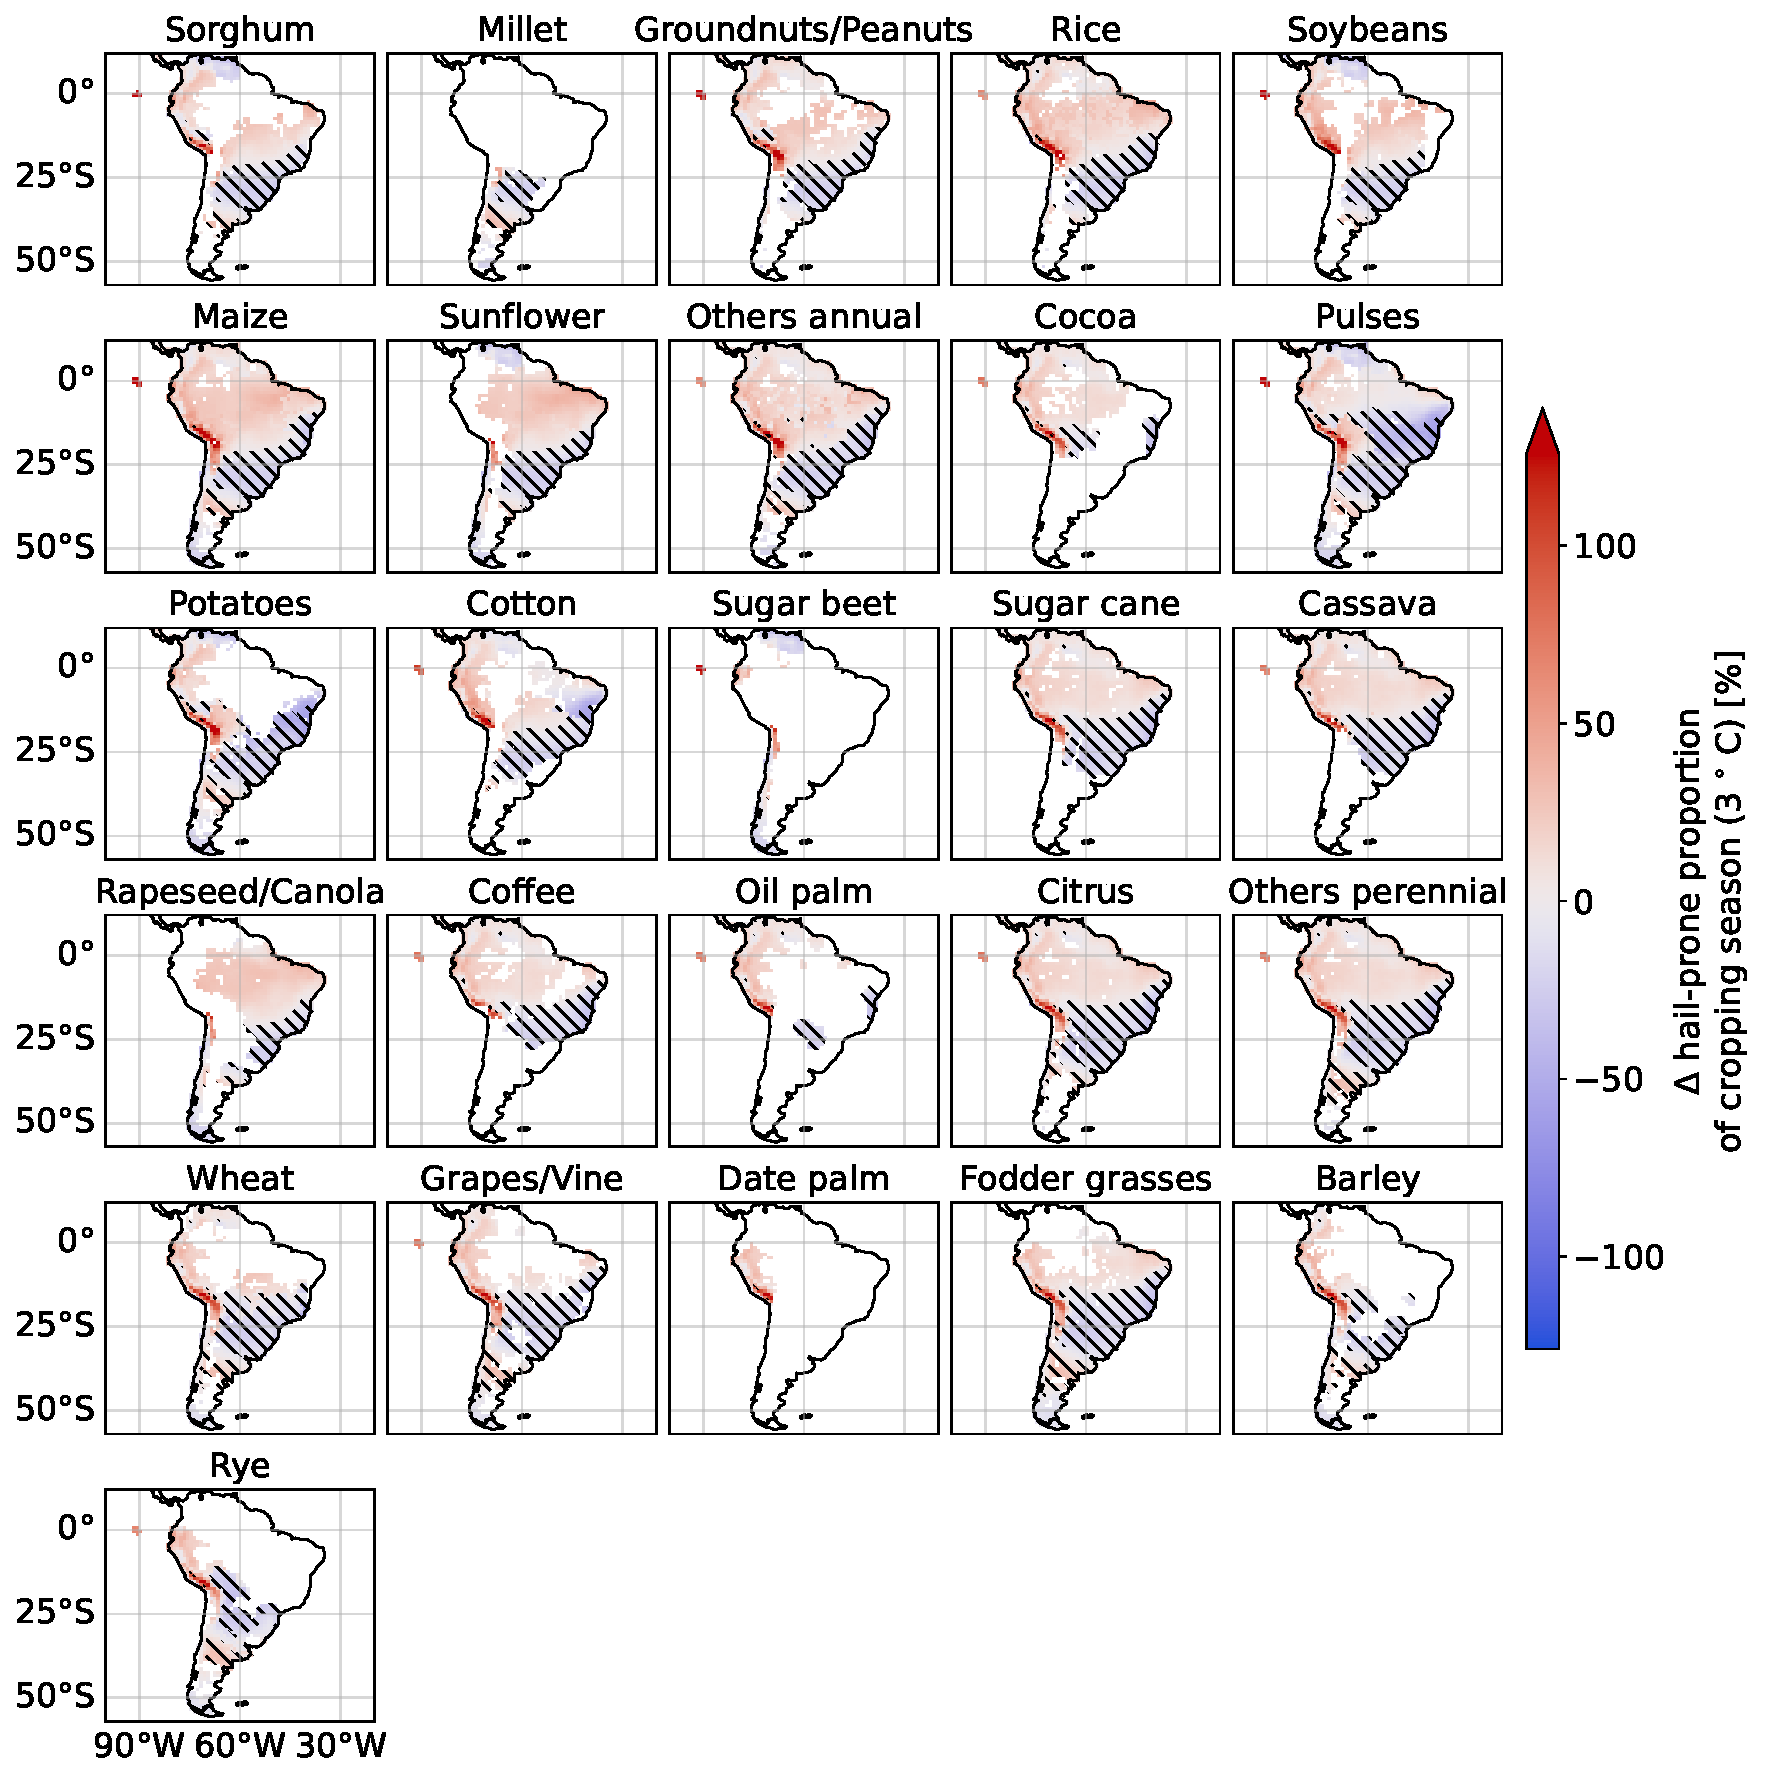
\includegraphics[width=\textwidth]{../../results/extended_data/crop_changes_south_america}
    \caption{As for Extended Data Figure \ref{fig:crop_changes_africa} but for
    South America.}
    \label{fig:crop_changes_south_america}
\end{figure*}

\FloatBarrier

\begin{table}
\begin{tabular}{lrrrrrrrrrrrrrr}
\toprule
Region & \multicolumn{2}{r}{Africa} & \multicolumn{2}{r}{Asia} & \multicolumn{2}{r}{Europe} & \multicolumn{2}{r}{Global} & \multicolumn{2}{r}{N. America} & \multicolumn{2}{r}{Oceania} & \multicolumn{2}{r}{S. America} \\
Epoch & 2\degr{} & 3\degr{} & 2\degr{} & 3\degr{} & 2\degr{} & 3\degr{} & 2\degr{} & 3\degr{} & 2\degr{} & 3\degr{} & 2\degr{} & 3\degr{} & 2\degr{} & 3\degr{} \\
Crop &  &  &  &  &  &  &  &  &  &  &  &  &  &  \\
\midrule
Barley & 329 & 341 & 725 & 1024 & 487 & 732 & 2735 & 3601 & 675 & 853 & 87 & 144 & 193 & 263 \\
Cassava & 1115 & 1064 & 463 & 601 &  &  & 2217 & 2256 & 154 & 157 & 18 & 20 & 460 & 404 \\
Citrus & 974 & 984 & 652 & 896 & 167 & 310 & 3165 & 3843 & 631 & 843 & 211 & 245 & 508 & 514 \\
Cocoa & 576 & 524 & 60 & 51 &  &  & 903 & 816 & 115 & 113 & 6 & 8 & 146 & 120 \\
Coffee & 774 & 763 & 410 & 522 &  &  & 1735 & 1800 & 161 & 165 & 18 & 20 & 360 & 318 \\
Cotton & 881 & 1074 & 731 & 892 & 127 & 210 & 2490 & 2960 & 315 & 341 & 122 & 136 & 312 & 304 \\
Date palm & 425 & 445 & 222 & 319 & 124 & 219 & 796 & 1037 & 16 & 40 &  &  & 8 & 7 \\
Fodder grasses & 121 & 167 & 1059 & 1337 & 511 & 727 & 3619 & 4516 & 887 & 1112 & 276 & 318 & 500 & 562 \\
Grapes/Vine & 293 & 340 & 713 & 942 & 373 & 569 & 2639 & 3394 & 433 & 614 & 146 & 177 & 422 & 485 \\
G.nuts/Peanuts & 764 & 862 & 645 & 727 & 82 & 152 & 2145 & 2454 & 275 & 307 & 73 & 91 & 306 & 310 \\
Maize & 860 & 976 & 776 & 998 & 307 & 501 & 3347 & 4189 & 709 & 926 & 119 & 147 & 320 & 375 \\
Millet & 792 & 901 & 647 & 838 & 61 & 171 & 1876 & 2437 & 55 & 92 & 74 & 94 & 92 & 157 \\
Oil palm & 606 & 558 & 296 & 415 &  &  & 1066 & 1129 & 57 & 56 &  &  & 107 & 100 \\
Others annual & 1050 & 1107 & 832 & 1054 & 383 & 652 & 3933 & 4837 & 875 & 1112 & 138 & 176 & 386 & 414 \\
Others perennial & 1317 & 1333 & 984 & 1258 & 544 & 776 & 4762 & 5652 & 846 & 1078 & 251 & 291 & 527 & 572 \\
Potatoes & 480 & 568 & 927 & 1092 & 429 & 662 & 3313 & 4172 & 821 & 1014 & 120 & 165 & 285 & 401 \\
Pulses & 745 & 851 & 938 & 1148 & 376 & 565 & 3616 & 4459 & 738 & 900 & 124 & 166 & 427 & 543 \\
Rapeseed/Canola & 16 & 22 & 463 & 809 & 314 & 507 & 1654 & 2318 & 365 & 436 & 66 & 102 & 210 & 192 \\
Rice & 930 & 971 & 555 & 645 & 123 & 254 & 2325 & 2638 & 294 & 324 & 18 & 36 & 348 & 344 \\
Rye & 3 & 21 & 401 & 638 & 396 & 600 & 1713 & 2582 & 453 & 684 & 95 & 152 & 125 & 242 \\
Sorghum & 819 & 946 & 626 & 819 & 191 & 322 & 2771 & 3502 & 499 & 666 & 132 & 172 & 285 & 328 \\
Soybeans & 389 & 442 & 848 & 959 & 258 & 396 & 2531 & 3032 & 487 & 625 & 62 & 85 & 239 & 267 \\
Sugar beet &  &  & 505 & 601 & 263 & 446 & 1001 & 1359 & 155 & 218 &  &  & 3 & 8 \\
Sugar cane & 981 & 969 & 514 & 666 & 58 & 103 & 2415 & 2588 & 259 & 276 & 115 & 122 & 479 & 431 \\
Sunflower & 222 & 311 & 757 & 877 & 280 & 428 & 2337 & 2925 & 467 & 644 & 91 & 110 & 277 & 302 \\
Wheat & 698 & 810 & 796 & 1220 & 470 & 670 & 3327 & 4399 & 609 & 802 & 132 & 196 & 383 & 457 \\
\bottomrule
\end{tabular}

\caption{Numbers of samples (grid points with significant changes) used to
generate each box plot in Figure \ref{main-fig:crop_changes}. ``N. America''
stands for North America, ``S. America'' for South America, and ``G.nuts'' for
groundnuts.}
\label{tab:bar_ns}
\end{table}

\end{document}
